\section{Evaluation}
\label{SEC:evaluation}


\section{Phase 1}

In our first phase of evaluation, our focus was quite simple: Did the tool
allow us to efficiently find environmental bugs? To measure efficiently, we
set out to answer the following questions:

\begin{enumerate}

\item{Do environmental bugs exist in widely used applications and can
      CrashSimulator find them? (Subsection~\ref{sec-env-bugs})}

\item{Do tests using CrashSimulator make yield too many false positives?
      (Subsection~\ref{sec-sorts-errors})}

\item{Can CrashSimulator
      execute tests efficiently? (Subsection~\ref{sec-perf})}

\end{enumerate}


\subsection{Do environmental bugs  exist in widely used applications and
can CrashSimulator find them?} \label{sec-env-bugs}

Do the types of bugs
identified by CrashSimulator exist in in popular applications?  This is a
crucial question to ask because,
if such bugs do not exist in practice, then there would be no need for
such a tool.  To test this premise,
we chose to look for two anomalies that we could test for in a large
array of programs.  One is a file system anomaly and the other is found in
network applications.
However, both use common API calls, and thus had the potential to
appear in many programs.  We selected the tested applications either
because they were deemed
``popular'' by Debian's Popularity Contest~\cite{DebPopCon}, or were from
GNU Coreutils.  Coreutils applications were chosen because of their
widespread inclusion in many Linux distributions.

\subsubsection{Unexpected File Types}
\label{sec-file-type-bugs}
Providing unexpected types of files to
applications.

The first anomaly investigated occurs when an application has to retrieve
and process data from a file.  Linux supports several ``special'' file
types apart from the standard ``regular'' file type, such as
directories, symbolic links, character devices, block devices, sockets, and
First-In-First-Out (FIFO) pipes.  While these special files
use the same system calls as regular files (such as {\tt read()} and
{\tt write()}), they behave in very different ways.  For example, {\tt
/dev/urandom} is a character device that produces an infinite amount of
pseudo-random data when read.  If an application that reads the full
contents of a file before processing it is provided {\tt /dev/urandom}, it
will fill memory or disk space and could
crash the system~\cite{YumAptEndless}.
Correct execution in these situations often requires applications
to examine the files in order to ensure they are of an appropriate type.

{\bf Method.}  Identifying these bugs involves changing an application's
execution trace to induce its response to an unexpected file type.  For
example, the {\tt sed} application, which modifies the contents of a text
file according to a provided command string, could be provided a symbolic
link, a directory, or a character device instead.  CrashSimulator
accomplishes this by identifying the calls to {\tt stat()}, {\tt fstat()},
or {\tt lstat()} that an application makes to examine the file, and then
changes the trace to simulate
one of the special file types.  If the application responds to
this injected information then there is the possibility that the special
file will be handled correctly.  On the other hand, if there is no
alteration in the behavior of the application,  then the condition is not
being handled correctly.

{\bf Findings.}
The results of this round of tests were shown in
Table~\ref{table:unexpectedtypes}.

For each application, CrashSimulator was invoked multiple times,and
the trace was modified
to simulate each of the non-standard file type anomalies.  Some
of the applications opened multiple files; in these cases each anomaly was
simulated for each of the file arguments to the application.
Table~\ref{table:unexpectedtypes} also shows the values that CrashSimulator
inserts into the return value of the {\tt stat()}-like call,
in response to
different file type anomalies.  A result of ``Initial Value'' indicates
that this is the file type the application was provided when the replayed
execution trace was recorded -- that is, a file of the type the application
was expecting.  A result of ``Recognizes'' indicates that the application
identified that it was being provided with an unexpected file type and its
execution diverged, indicating that it was potentially handling the
unexpected file type correctly.  A result of ``Fail'' indicates that the
application failed to recognize the presence of the unusual file type
because execution never diverged from the trace being replayed.  We
manually examined a subset of the listed application behaviors simulated by
CrashSimulator and verified they were consistent with the actual behavior
on the given file type.

\begin{table*}[t]
    \scriptsize{}
    \begin{tabular}{l  l  |  l  l  l  l  l  l  l}
    \toprule{}
        Application & Condition Tested           & IFREG        & IFDIR        & IFCHR     & IFBLK    & FIFO      & IFLNK    & IFSOCK\\
\hline
        {\tt Aspell}      & Dictionary File            & Initial Value  & Fail           & Recognizes  & Fail       & Fail        & Fail       & Fail\\
        {\tt Aspell}      & File being checked         & Initial Value  & Fail           & Recognizes  & Fail       & Fail        & Fail       & Fail\\
        {\tt gnu-gpg}     & secring.gpg                & Initial Value  & Fail           & Fail        & Fail       & Fail        & Fail       & Fail\\
        {\tt vim}         & File being opened          & Initial Value  & Recognizes     & Recognizes  & Recognizes & Recognizes* & Recognizes & Fail\\
        {\tt nano}        & File being opened          & Initial Value  & Recognizes     & Recognizes  & Recognizes & Fail        & Fail       & Fail\\
        {\tt sed}         & File being edited          & Initial Value  & Fail           & Recognizes  & Fail       & Fail        & Fail       & Fail\\
        {\tt df}          & /proc                      & Fail           & Initial Value  & Fail        & Fail       & Fail        & Fail       & Fail\\
        {\tt wc}          & File being checked         & Initial Value  & Recognizes     & Recognizes  & Recognizes & Recognizes  & Recognizes & Recognizes\\
        {\tt du}          & Directory being checked    & Recognizes     & Initial Value  & Recognizes  & Recognizes & Recognizes  & Recognizes & Recognizes\\
        {\tt install}     & File being installed       & Initial Value  & Recognizes     & Fail       & Fail      & Fail       & Recognizes & Fail\\
        {\tt fmt}         & File being formatted       & Initial Value  & Fail          & Recognizes  & Fail      & Fail       & Fail      & Fail\\
        {\tt od}          & File being dumped          & Initial Value  & Fail          & Recognizes  & Fail      & Fail       & Fail      & Fail\\
        {\tt ptx}         & File being read            & Initial Value  & Recognizes     & Recognizes  & Recognizes & Recognizes  & Recognizes & Recognizes\\
        {\tt comm}        & Second file being compared & Initial Value  & Fail           & Recognizes  & Fail       & Fail        & Fail       & Fail\\
        {\tt pr}          & File being read            & Initial Value  & Fail           & Fail        & Fail       & Fail        & Fail       & Fail\\
\hline
        {\tt readlink}    & Link being evaluated       & \textbf{No file checks performed} & & & & & & \\
        {\tt unlink}      & File being unlinked        & \textbf{No file checks performed} & & & & & & \\
    \bottomrule{}
    \end{tabular}
    \caption{Applications tested for their handling of unexpected file types.}
    \label{table:unexpectedtypes}
\end{table*}

The frequency of failed executions in our results indicate that many
applications make the assumption that they will only be used to process
regular files.  When this assumption does not hold, execution results
can be hard to predict.  In many cases a denial of
service condition occurs in the form of the application ``hanging,'' as it
attempts to incorrectly process the file.  This may happen harmlessly, such
as if an application blocks forever waiting for a {\tt read()}
call to retrieve non-existent data from an empty FIFO, or harmfully, as
when an application attempts to read in and process an
``infinitely large'' file, that will eventually fill all
available memory or disk
space~\cite{Cappos_CCS_08}.

Of particular interest is the behavior we see in the last two applications
listed in Table~\ref{table:unexpectedtypes}.  Each application correctly
recognized when an unexpected file type was encountered, as they
are simply ``dumb'' wrappers around the system calls
with which they share a name.  As such, they essentially,
they just hand the specified
file to their corresponding system call and, in the case of an error, use
{\tt perror()} to print the correct localized error message.  In short,
these applications pass their error handling responsibilities to the
kernel.

\begin{table}[t]
    \scriptsize{}
    \begin{tabular}{l  l  l  l  l  l  l  l  l}
    \toprule{}
        Application         & IFDIR                     & IFCHR       & IFBLK                & FIFO \\
\hline
        {\tt wc}            & Error: Is a Directory     & hangs       & slowly process file  & Hangs\\
        {\tt install}       & Error: Omitting Directory & Fills disk  & slowly copies file   & Hangs\\
        {\tt fmt}           & No output                 & hangs       & garbage output       & Hangs\\
        {\tt od}            & Error: read error         & hangs       & No output            & Hangs\\
        {\tt ptx}           & Error: Is a Directory     & fills disk  & garbage output       & Hangs\\
        {\tt comm}          & Error: Is a Directory     & hangs       & garbage output       & Hangs\\
        {\tt pr}            & Error: Is a Directory     & hangs       & garbage output       & Hangs\\
\hline
    \bottomrule{}
    \end{tabular}
    \caption{Responses of a sample of coreutils applications when exposed to
      anomalous conditions.  The IFCHR file used was the infinite-length {\tt
        /dev/urandom}.}
    \label{table:applicationresponses}
\end{table}


In order to confirm the accuracy of CrashSimulator's assessments we manually
exposed a subset of the Coreutils applications we tested to the unusual file
types to get an idea of how they would respond.
Table~\ref{table:applicationresponses} contains the results of this test.
CrashSimulator's evaluation of an application can map to real world bug behavior
in a few different combinations
One
possibility is that CrashSimulator asserts that the application will fail
and in practice it does.  This is the case when we evaluated
the response of  {\tt install} when it was provided a character device
rather than a regular file. CrashSimulator predicted failure and the
application ended up filling the disk of the machine on which it was run.  The
opposite can also occur.  That is, CrashSimulator reports that the
application detected the anomalous condition and the application manages to
do so in practice,  as when we evaluated {\tt wc}'s response to
being run on a directory.

There were however, a few times when CrashSimulator and the
application's response disagreed.  This
happened when we evaluated {\tt ptx}'s response to an
infinite-sized character device.  CrashSimulator reported that {\tt ptx}
had correctly responded to the anomaly.  But in reality, {\tt ptx} filled the
disk of the the test machine.  As will be discussed later, correcting this
error is easily accomplished by improving the checker used in this
assessment -- an effort similar to updating a unit test when it is shown to
be incomplete.  Overall, the results of this ``real world'' analysis
support the claim that CrashSimulator can identify real bugs that can have
damaging consequences.

\subsubsection{Slowloris attack} Delaying network applications for extended
periods.


The second anomaly we examined involves an application's behavior when it
attempts to communicate over a network with extremely long (on the order of
minutes) response times.  At a low level, applications retrieve data from a
network socket by waiting for data to be available and then reading it.  A
key aspect of this approach is handling the situation where communication
takes too long and should time out.

{\bf Method.} CrashSimulator can detect whether an application is
vulnerable to this attack by modifying the trace to simulate large
amounts of time elapsing between network operations.  In this approach,
CrashSimulator determines whether or not the application makes any effort
to configure its network communications with a timeout value. This is done
by examining the presence or absence of {\tt setsockopt()}, {\tt poll()}
and {\tt select()} calls as well as the timeout values that may or may not
have been passed to them. Applications that do not set the timeout are
subject to the operating system-defined protocol timeout value (19 minutes
on Linux).  Note that by properly manipulating the results of all
time-returning calls, CrashSimulator can simulate an execution where close
to the maximum timeout value occurs, without actually spending any time
waiting.


Again, our selection of network applications and libraries were based on
those that were
most popular on Debian's ratings~\cite{DebPopCon}.

\begin{table}[t]
  \scriptsize{}
  \begin{tabular}{l | l}
    \toprule{}
    {\bf Application}              & {\bf Analysis Result}\\
    {\tt wget}                     & Overly long timeout supplied to {\tt select()} \\
    {\tt ftp}                      & No {\tt poll()} or {\tt select()}, no timeout set \\
    {\tt telnet}                   & {\tt select()} specifies no timeout \\
    {\tt urllib http}              & No {\tt poll()} or {\tt select()}, no timeout set \\
    {\tt urllib ftp}               & No {\tt poll()} or {\tt select()}, no timeout set \\
    {\tt ftplib}                   & No {\tt poll()} or {\tt select()}, no timeout set \\
    {\tt httplib}                  & No {\tt poll()} or {\tt select()}, no timeout set \\
    {\tt requests}                 & No {\tt poll()} or {\tt select()}, no timeout set \\
    {\tt urllib3}                  & No {\tt poll()} or {\tt select()}, no timeout set \\
    {\tt python-websocket-client}  & No {\tt poll()} or {\tt select()}, no timeout set \\
    \bottomrule{}
  \end{tabular}
  \caption{Applications tested for their handling of extremely slow response
    times from the host with which they are communicating }
  \label{table:slowloris}
\end{table}


{\bf Findings.} As Table~\ref{table:slowloris} shows, all of these
applications were vulnerable to this sort of anomaly, with timeouts taking
hours or even days in some cases to resolve.
What's more, in the vast majority of
cases, the problem occurs because the application makes no effort to
specify a timeout value.  This means an attacker can transmit one byte of
data per timeout period (per Linux's value of 19 minutes for TCP sockets),
allowing them to keep the application alive instead of quitting.


This attack technique has been effectively exploited in the wild.  The {\tt
slowloris} tool allows a single attacking host to successfully deny service
to a vulnerable web server with minimal bandwidth usage by simply
introducing delays between the headers sent to the victim by an attacking
HTTP client.  Because many web servers at the time  of {\tt slowloris's} release
allowed large timeouts
between messages from the clients, one web client could effectively tie up
the resources of a web server for a long period of time.
This can cause a slow buildup of unending or long lived jobs that consume
resources and cause detrimental system behavior~\cite{Slowloris}.
Similar attacks can be used to indefinitely delay security updates to
clients, leaving them vulnerable to compromise~\cite{Cappos_TR_08}.

{\bf Concluding Thoughts} The results of the above analysis show that
CrashSimulator is readily able to identify novel bugs in widely used
applications, including security-focused applications like gnu-gpg, and a host
of popular network applicaitons, by following a repeatable and principled
protocol.


\subsection{What sorts of errors does CrashSimulator make?}
\label{sec-sorts-errors}

\preston{This false positives section needs to be reworked as it is based on
"checkers" that could run without all of CrashSimulator's machinery.  We
received negative feedback about this.}

The primary source of false positives in CrashSimulator is an application
using a different sequence of system calls to implement a given operation
than a checker was anticipating. CrashSimulator's approach allows these
situations to be easily corrected, once identified through analysis of the
incorrect test results.  This is similar to the circumstance where an
application's test suite is missing a test, necessitating action by the
developer to construct the missing test.

For example, consider GNOME's {\tt glib} file handling facilities.  When an
application makes use of these facilities to move a file across storage
devices the library itself correctly handles the behaviors described above
for a ``correct'' file move operation.  When we used CrashSimulator with
the checkers described above to analyze a minimal application that used
{\tt glib} for a cross-device move, we got reports stating that the
application {\em did not} respond correctly to the anomaly.  By manually
examining a system call trace, we found that, while {\tt glib} correctly
performs the required behaviors, it does so using alternative system call
sequences.  Rather than using a sequence of {\tt read()} and {\tt write()}
calls, as our checker expected, {\tt glib} creates a pipe and uses the {\tt
splice()} system call to copy the contents out of the source file, through
the pipe and into the destination file.

Fortunately, as soon as false positives like this are discovered,
CrashSimulator's checkers can be modified to deal with alternative
approaches to handling an anomaly.  This approach is viable because there
are a finite number of system calls, and a given operation can be mapped to
a manageable subset of system calls.  Given the above example around moving
files, consider the mapping from high level ``operation'' to the set of
system calls that can implement it in Table~\ref{table:stepsandcalls}.
Each of the steps in the operation map to a small number of system calls
and, in most cases, only one of these system calls is necessary.  In
situations where two system call sequences can correctly implement the same
operation, CrashSimulator simply runs two checkers in parallel and accepts
the execution if either one ends in an accepting condition.

\begin{table}[t]
    \scriptsize{}
    \begin{tabular}{l | l }
    \toprule{}
      {\bf Operation}                                               & {\bf Potential System calls}\\
      Examine source file                                     & stat64(), lstat64(), fstat64()\\
      Examine destination file                                & stat64(), lstat64(), fstat64()\\
      Open source file                                        & open()\\
      Read contents of source file                            & read(), splice() with a pipe\\
      List source file's & \\ ~~~~~extended file attributes             & listxattr(), llistxattr(), flistxattr()\\
      %Read contents of source file's extended file attributes & getxattr(), lgetxattr(), fgetxattr()\\
      Read contents of source file's                    & \\
      ~~~~~~~extended file attributes & getxattr(), lgetxattr(), fgetxattr() \\
      Open destination file                                   & open(), optionally unlink() the file first\\
      Write contents to destination file                      & write(), splice() with a pipe\\
      Apply extended file attributes to & \\ ~~~~~destination file      & setxattr(), lsetxattr(), fsetxattr()\\
      Apply proper timestamps to & \\ ~~~~~destination file             & utimens(), futimens()\\
      Apply proper permissions & \\ ~~~~~to destination file            & chmod(), open() with a modeline specified\\
      Close the source file                                   & close()\\
      Close the destination file                              & close()\\
    \bottomrule{}
    \end{tabular}
    \caption{Each step of a successful cross-disk file move operation mapped to
      the system call or calls that can implement it}
    \label{table:stepsandcalls}
\end{table}

\subsection{Can CrashSimulator execute tests efficiently?}
\label{sec-perf}


One key attribute of successful testing tools is that they are able to
complete their tests in a timely manner.  If a tool takes too long
, users will be less likely to run it, which reduces its
usefulness dramatically. To this end, the performance of CrashSimulator was
evaluated in order to determine whether or not it was able to complete its
test executions in an acceptable time frame.

{\bf Method.} To determine the efficiency of CrashSimulator as a testing tool,
we examined the completion
times for executions of the specified application in both
native and replay execution modes.


    \begin{figure}[t]
        \center{}
        \fbox{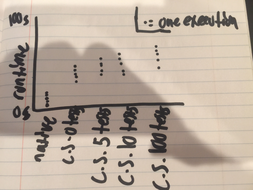
\includegraphics[scale=.75]{performance.png}}
        \caption{\emph{This shows the run time difference between the
native program and CrashSimulator in seconds.  Each dot indicates an
        execution.  The X axis shows time values for native executions, and
        executions under CrashSimulator with 0, 5, 10, and 100 tests
        performed respectively.
}}
         \label{figure:performance}

    \end{figure}


{\bf Findings.} Overall, the performance of CrashSimulator is usually
about an order of magnitude slower than if the original program is executed
natively.  This is largely due to performance problems in our (unoptimized)
prototype, primarily our utilization of Python and {\tt ptrace} once
process sets have been liberated from {\tt rr}.  Tracing the program
with {\tt ptrace} adds up to a factor of 5x in overhead,  which could be
removed with more efficient mechanisms like {\tt eBPF} or a loadable kernel
module.  In addition, starting up the Python interpreter increases the
startup time of our prototype's supervisor.

Though aspects of our performance were less efficient than desired, its
ability to execute many tests throughout the course of one replay and the
lack of blocking while waiting for test completion somewhat makes up for
this slowness. In some cases CrashSimulator will be more efficient than
running the program natively since {\tt rr's} replay does not require
actual execution of most system calls.  This means that CrashSimulator
avoids the system call overheads, such as I/O.

\preston{We probably want to keep this point, but I agree that it doesn't fit
here}
Note also that natively testing the timeout of networked applications (not
shown) would take an extended period of time, at least as long as the
allowed timeout value.  CrashSimulator avoids this cost by simulating the
fact that time has progressed for future system calls.

Overall, these results indicate that CrashSimulator is able to replay
executions in a performant manner.  Figure~\ref{figure:performance} shows
that the majority of the above executions completed around an order of
magnitude slower than their native counterparts.  CrashSimulator's
asynchronous testing means that enabling additional tests does not
significantly degrade performance as long as multiprocessing resources are
available on the system.


\section{Phase 2--Tool Usability Evaluation}

Satisfied that CrashSimulator's technique can reliably identify bugs in
real world applications, we turned our focus toward determining how well it
could be used by the larger developer community.  In this evaluation phase
we conducted a user study in hopes of answering the following questions:

\begin{enumerate}

\item Are users able to effectively find bugs using CrashSimulator?

\item Does CrashSimulator allow users to test specific application areas?

\item Does CrashSimulator allow its users to efficiently construct a test suite?

\item Does user experience level have an impact on their ability to use the
tool?

\item Does CrashSimulator provide output that is useful in locating and
fixing bugs?

\end{enumerate}

\subsection{Study Design}

We gathered a group of YYYY participants from a computer science master's
program.  These students had varying backgrounds in relation to software
development and automated testing.  All received AAA hours
of training on each of these tools.  This training focused on the tools'
initial setup, configuration, and usage,
as well as on how to interpret its
results.  BBB of the students had used AFL in previous course work.  None
of the students had previous experience with Mutiny or CrashSimulator.

We asked our participants to test popular real-world applications with the
goal of identifying new bugs and reporting them to the application's
developers.  In performing this task our participants had to correctly set
up and configure each of the tools, execute a testing process, evaluate the
results, and produce a sufficient proof of validity for each bug to
convincingly support the case for fixing it.  Each of these steps is an
opportunity to for gain insight into how CrashSimulator stacks up against
other tools.

We used three techniques to capture the experience of our participants as
they used the tool.  First, we examined the time required for participants
to perform each step of the process of finding and reporting a bug.
This data, along with hard counts of the number of bugs identified by our
participants using each of the tools, provided a quantitative measure of
each tool's usability.

To measure qualitative concerns,
participant impressions were gathered using
several instruments.  First, data on developer skills and educational
backgrounds was gathered using a pre-study survey.
Second, during the three week
study period, the participants' progress toward finding and fixing bugs was
tracked through the submission of weekly update worksheets.  Finally, at
the end of the study period, overall developer impressions were gathered
using a post-survey and one-on-one interviews.  These instruments were
structured to give insight into how CrashSimulator compares to the other
tools in three areas:

\begin{itemize}

\item Usability of the tool. (i.e. set up, configuration, executing tests,
interpretring results)

\item Extendability of the tool through the creation of additional
anomalies

\item Effectiveness of the tool in its ability to test specific areas of
interest in an application.

\end{itemize}

\subsection{Tools Selected for Comparison}


CrashSimulator's system call based technique allows its user to replicate
anomalous environmental conditions in a wide variety of operating systems
domains.  As was discussed earlier, we used this capability to test
applications' responses to unusual filesystem and network conditions.
In light of this it
is appropriate to compare CrashSimulator against two existing testing
tools, one that is file based (AFL) and another that performs network
oriented testing (Mutiny).

\begin{itemize}

\item{AFL} (American Fuzzy Lop) is a file-based fuzzer that tests an
application by mutating the contents of a candidate file provided by
the user.  It offers two improvements over the naive approach of simply
passing random data to an application through a file.  First, AFL
bases its mutations on a valid file for the application.  This
increases the chance that the mutated file will not be immediately rejected
by
processing code, which improves coverage.  Second, AFL provides a set of
C compiler customizations
that at compile time add instrumentation code to the
application being tested.  This instrumentation
allows AFL to tune its mutations to more thoroughly exercise the
application's code paths.  The intention when testing with AFL is
to generate an input file that makes the application crash.  Once a
crash-causing file is discovered, users must manually analyze the
file and application in order to ascertain the cause of the crash
and fix it.  Though there is some support for testing closed source
applications through a hypervisor AFL, is intended to test
applications written in C on Linux and has an impressive track
record in terms of bugs discovered in major applications that meet
this criteria.

\item{Mutiny Fuzzer} At a high level, Mutiny has an architecture similar to
CrashSimulator.  Its primary method of interacting with an application
is mutating and replaying previously captured {\tt pcap} recordings
of network activity.  The specific mutations to be made are encoded
as mutator plugins that are enabled and disabled by the tool's
user.  Mutiny monitors and takes action based on the application's
behavior during replay of a mutated recording.  For example, Mutiny
can alter the data being communicated to the target host when a
particular network error is encountered.

\end{itemize}


\subsection{Are users able to effectively find bugs using CrashSimulator?}

For any testing tool, the primary concern is whether or not it can find
bugs.  To evaluate this concern in the case of CrashSimulator, case we need
to answer users are able to effectively find bugs in real world
applications.  To focus this process on the actual but finding and fixing
process, rather than open source development meta-concerns, participants
were encouraged, but not limited to, testing applications listed highly on
the Debian popularity contest.  These applications are more likely to have
clean, mature code bases and active developer communities reducing the
barrier to entry for our participants.

{\bf Findings. }

A total of 15 bugs were found using CrashSimulator, and, perhaps not
surprisingly, the majority were reported by participants with a
self-reported high degree of operating systems experience.
~\ref{table:fig-tool-exp} contains the
counts of bugs identified during the study broken down by
the tool used to identify them, as well as developer's self reported
developer experience level with operating system concepts.
Participants with a moderate and low degrees of operating
systems experience found more bugs AFL.  Participant impressions indicated
that, while AFL was easier to set up, the ``luck'' aspect of hoping to come
across a crash-causing input mutation was unsatisfying.  In spite of this,
EEEE bugs were found using AFL.  Survey results indicate that lower bug
counts for Mutiny can be attributed to the increased complexity of setting
up an environment where valid network recordings could be taken.  Overall,
fewer network applications were tested.

\begin{figure}[t]
  \center{}
  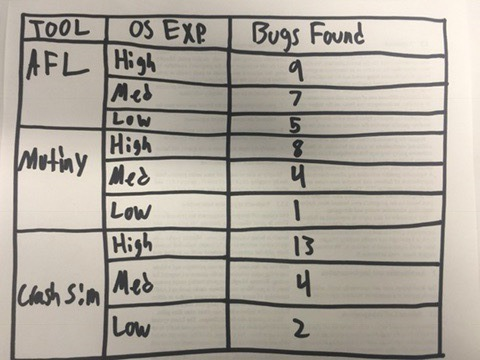
\includegraphics[scale=.5]{images/table1}
  \caption{\emph{Bugs Found by Tool and Experience Level}}
  \label{fig-tool-exp}
\end{figure}


{\bf Discussion. }

The above results indicate that, when it comes to using CrashSimulator,
having experience with operating systems concepts is very beneficial.  At
the same time, users with a self-reported low degree of experience with OS
concepts were still able to identify bugs by using its built in corpus of
anomalies. ~\ref{table:fig-tool-anomaly} shows which
of these anomalies most commonly
resulted in application bugs.

\begin{figure}[t]
  \center{}
  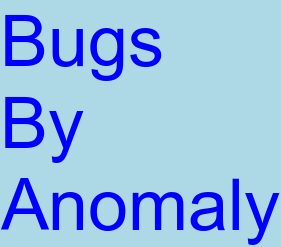
\includegraphics[scale=.5]{images/anomaly}
  \caption{\emph{Bugs Found Using CrashSimulator Organized by Anomaly}}
  \label{fig-tool-anomaly}
\end{figure}


{\bf Discussion on Specific Bugs. }

\preston{I don't have text here because I feel like I'd be making it up
entirely and it would likely all be thrown away.  However, if having some
stuff here is useful let me know and I'll come up with some.}


\subsection{Does CrashSimulator allow users to test specific application
areas?}

\preston{The more I read this the less I like this question.  What I want
to figure out is how many participants don't prefer/are unable to the tool
because it is too low level or not appropriate for testing the parts of
applications they are concerned with.  For example, a student that is
mostly concerned with user-space data processing code that isn't testable
by CrashSimulator}

Modern applications typically consist of many different parts (e.g. user
interfaces,  back-end processing, storage, networking) and may require
different skill sets to operate effectively.  These different application
areas also require disparate testing strategies.  For example, some
application areas such as graphical user interfaces, are notoriously
difficult to cover depending on the tools and techniques being used.  These
difficulties usually result from limitations in the way the testing tool
interacts with the application. We wanted to know whether or not
CrashSimulator was able to effectively test the specific areas of
applications its users needed to evaluate.  To answer this question, we
turn to the surveys our participants completed regarding their experience
with CrashSimulator.


{\bf Findings. }

The results from our surveys indicate that a strong correlation between our
participants' self-reported
backgrounds and what areas of an application they tested.
Participants with lower self-reported development experience focused more
on more surface level concerns, and so they preferred the simple
process of providing an input file to AFL as opposed to using
CrashSimulator's more complex
setup.  Participants with little native development experience struggled
with deciding which anomalies were appropriate to apply to the applications
they were evaluating.  For this reason, there were instances of tests
being run that
didn't accomplish anything.  We hope to reduce cases like this in the
future by providing a more helpful interface for selecting anomalies.

A majority of participants
with a high degree of experience in software engineering tended
to focus on testing an application's interaction with various library and
APIs provided by operating systems.
Survey results indicate participants were
satisfied with CrashSimulator's ability to test applications' interaction
with file and network APIs.


{\bf Discussion. }

Findings indicate that a higher level of software development experience
tends to push participants towards testing interfaces between modules in an
application.  This resulted in overall higher satisfaction with
CrashSimulator amongst these participants.  It should be noted that several
developers found bugs in the libraries on which the applications they were
testing depended.  Being able to localize a bug to a specific sequence of
system calls means that these participants were saved the effort of
analyzing application code for a bug whose cause lay elsewhere.

Users with less self-reported software engineering experience expressed
some concern with CrashSimulator's limitations around testing the user
facing aspects of applications.  For example, CrashSimulator requires more
up front effort than tools like AFL when conducting simple
tests, such as mutating the properties of an input file.


\subsection{Does CrashSimulator allow its users to construct a test suite
efficiently?}

Constructing a test suite using CrashSimulator involves identifying new
anomalies to test for and creating the mutators required
to test an application's response to them.
The effort and skill involved in
this process is similar to that involved in writing a unit test or
integration test using a modern testing framework.  However, unlike a unit
test or integration test, a CrashSimuator test can be run
against multiple
applications without concern for dependencies like the language in which
they were
written in or the libraries they depend on.


{\bf Findings. }


Most developers reported a high degree of
satisfaction with regard to the speed
of setup for AFL.  In contrast, there was a concensus that
CrashSimulator required an
overall higher initial outlay of effort before testing could begin.
Additionally, they indicated that expanding a CrashSimulator test suite by
implementing new checkers and mutators was more difficult that either
expanding the scope of fuzzing with AFL or instructing Mutiny to mutate
different messages from a recorded network session.  However, the subjects
did appreciate
CrashSimulator's ability to allow for
more specific testing,
to test across multiple applications
with minimal additional effort once the tests had been constructed.

Those participants who preferred to test a wide variety of applications
quickly were inclined to reach first for AFL.  Survey results indicated
that this was due to the tool's ease of use and lack of configuraiton.
This allowed participants to quickly begin and halt testing an application
without concern for recovering their initial outlay of effort.  However,
those participants
who wanted to dive deeply into a smaller set of applications
preferred CrashSimulator and Mutiny to AFL.  There was a great deal of
positive feedback around CrashSimulator's ability to use a mutator to apply
an anomaly to multiple eligible system call sequences throughout an
execution.  This meant a single test could be constructed to cover similar
operations throughout an application's code base, which would
shrink the size of the
required test suite in the process.


{\bf Discussion. }

There is no direct comparison to CrashSimulator's "test writing"
process in AFL, which
uses built in rules and patterns to mutate input files.  Our
findings indicate that this is either a blessing or a curse
depending on the
a user's preferred testing style.  CrashSimulator certainly requires
more initial effort but it can be paid back many fold if multiple
applications are tested using the same tests.


\subsection{Does user experience level have an impact on ability to use the
tool?}

The background of a user can
dramatically influence their experience with a
tool.  In answering this question we hope to ascertain whether
CrashSimulator requires its users to
have significant skills in a particular
area in order to use it effectively. ~\ref{table:fig-skill-exp}
compares our participants
self-reported skillsets to their positive or negative experiences with
CrashSimulator.


{\bf Findings. }

\begin{figure}[t]
  \center{}
  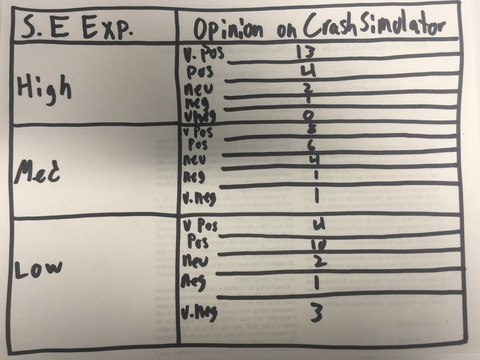
\includegraphics[scale=.5]{images/table2}
  \caption{\emph{Skill Level Compared to User Experience.}}
  \label{fig-skill-exp}
\end{figure}

As can be seen in Table 2, a strong background in operating systems
concepts correlates with a more satisfactory user experience with
CrashSimulator.  This is almost certainly because users who understand the
operation of system calls are able to quickly understand and utilize the
anomalies provided with CrashSimulator.  Additionally, these users were
more likely to identify their own anomalies and construct their own
mutators, which resulted in more bugs being found.

Interestingly, some participants who reported less familiarity in operating
systems did have a positive experience with CrashSimulator.
Surveys indicated
that these participants relied more heavily on built-in
anomalies and mutators.  These bugs were less likely to be fixed once
identified but, in spite of this, ZZZ new bugs were reported to projects'
developers.


{\bf Discussion. }

Given the level with which CrashSimulator interacts with applications, it
is not surprising that users with significant operating systems backgrounds
are better able to utilize the tool's more advanced features.  The
advantage of CrashSimulator in this case is that the expertise of one
high-level user
could be utilized by the rest of a development team through the sharing of
anomalies and mutators.

It is encouraging to see that users with limited operating systems
background had success
with the tool.  Based on this, we believe it is likely that CrashSimulator
could be successfully adopted by real-world teams whose members have
diverse background skillsets.  Users that are more comfortable with the
concepts CrashSimulator relies on can supply new testing materials as
needed while other users can rely on the portable nature of
these tests to evaluate new applications without
having to worry about their implementation details.


\subsection{Does CrashSimulator provide output that is useful in locating
and fixing bugs?}


{\bf Findings. }

Participant feedback across the board indicated that CrashSimulator's
output made it easier to identify bugs than the simpler crash reports
provided by AFL and Mutiny.  This impression is backed up by the results in
~\ref{table:fig-fixed-tool} that
show a higher percentage of bugs identified with
CrashSimulator were fixed than bugs identified with the other tools.

In a few cases participants lamented having put considerable effort into
identifying the source of bugs found with AFL and Mutiny without result.
This is somewhat confounded by these participants having typically reported
lower experience with debugging tools, operating systems concepts, and
software development in general.


\begin{figure}[t]
  \center{}
  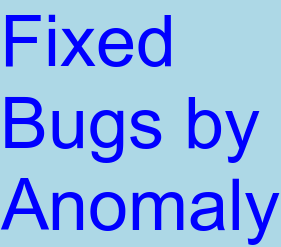
\includegraphics[scale=.5]{images/table3}
  \caption{\emph{Identified Bugs With Accepted Fixes By Tool}}
  \label{fig-fixed-tool}
\end{figure}


{\bf Discussion. }

There are two reasons, other than output quality, that bugs found with
CrashSimulator were more likely to be fixed -- bug "depth" and the ease
with which a bug can be fixed.  It is possible that, because CrashSimulator
focuses on anomalies in an applications environment, a source of bugs that
is not well tested in most applications, a higher number of easily fixed,
low
hanging fruit style bugs were identified compared to the more battle tested
user input handling code paths that AFL and Mutiny tend to explore.
Additionally, many of the bugs types identifiable with CrashSimulator arise
because of a minor missing check meaning that the fix is small and easily
incorporated.
